\documentclass[11 pt]{article}
\linespread{1.2}

%Paquete para que Tex acepte caracteres no ASCII
\usepackage[utf8]{inputenc}

%Paquete de colores
\usepackage{xcolor}
	\definecolor{codepurple}{RGB}{162, 112, 184}
	\definecolor{codegray1}{RGB}{180,180,180}
	\definecolor{codegray2}{RGB}{250,250,250}
	\definecolor{codered}{RGB}{200,27,50}
	\definecolor{codegreen}{RGB}{20,180,80}
	\definecolor{codeblue}{RGB}{14,126,196}
	\definecolor{codeyellow}{RGB}{240, 210, 45}

%Paquete de gráficos en figuras (fotos, tablas...)
\usepackage{graphicx}

%Paquete para escribir código
\usepackage{listings}
	\lstdefinestyle{mystyle}{
		frame=top,frame=bottom,
    backgroundcolor=\color{codegray2},   
    commentstyle=\color{codepurple},
    keywordstyle=\color{codered},
    numberstyle=\tiny\color{codegray1},
    stringstyle=\color{codeblue},
    basicstyle=\ttfamily\scriptsize,
    breakatwhitespace=false,         
    breaklines=true,                 
    captionpos=t,                    
    keepspaces=true,                 
    numbers=left,                    
    numbersep=5pt,                  
    showspaces=false,                
    showstringspaces=false,
    showtabs=false,                  
    tabsize=2
	}
	\lstset{
		style=mystyle,
		language=Ruby,
     literate=
         {á}{{\'a}}1
         {í}{{\'i}}1
         {é}{{\'e}}1
         {ú}{{\'u}}1
         {ó}{{\'o}}1
         {Á}{{\'A}}1
         {Í}{{\'I}}1
         {É}{{\'E}}1
         {Ú}{{\'U}}1
         {Ó}{{\'O}}1
         {ñ}{{\~{n}}}1
         {Ñ}{{\~{N}}}1
  }
	\renewcommand{\lstlistingname}{Listado}

%Controlar el layout de enumerize, itemize y description
\usepackage{enumitem}
	\setlist[itemize]{label={$\varnothing$}}
	
%Paquetes de notación matemática
\usepackage{amsmath}
	\DeclareMathOperator{\Ima}{Im}
	\DeclareMathOperator{\Nuc}{N}
	\DeclareMathOperator{\Int}{Int}
	\DeclareMathOperator{\Vol}{Vol}
	\DeclareMathOperator{\masa}{masa}
	\DeclareMathOperator{\traza}{tr}
	\DeclareMathOperator{\adjunta}{adj}
	\DeclareMathOperator{\grado}{gr}
	\DeclareMathOperator{\Dom}{Dom}
	\newcommand{\innprod}[2]{\left< #1 , #2 \right>}
	\newcommand{\conj}[1]{\overline{#1}}
	\newcommand{\der}[2]{\frac{d #1}{d #2}}
	\newcommand{\pder}[2]{\frac{\partial #1}{\partial #2}}
	\newcommand{\abs}[1]{\left\lvert #1 \right\rvert}
	\newcommand{\norm}[1]{\left\lVert #1 \right\rVert}
	\makeatletter
	\renewcommand*\env@matrix[1][\arraystretch]{%
 	 	\edef\arraystretch{#1}%
  	\hskip -\arraycolsep
  	\let\@ifnextchar\new@ifnextchar
  	\array{*\c@MaxMatrixCols c}}
  \newcommand{\xRightarrow}[2][]{\ext@arrow 0359\Rightarrowfill@{#1}{#2}}
	\makeatother
	\def\upint{\mathchoice%
    {\mkern13mu\overline{\vphantom{\intop}\mkern7mu}\mkern-20mu}%
    {\mkern7mu\overline{\vphantom{\intop}\mkern7mu}\mkern-14mu}%
    {\mkern7mu\overline{\vphantom{\intop}\mkern7mu}\mkern-14mu}%
    {\mkern7mu\overline{\vphantom{\intop}\mkern7mu}\mkern-14mu}%
  	\int}
	\def\lowint{\mkern3mu\underline{\vphantom{\intop}\mkern7mu}\mkern-10mu\int}
	
\usepackage{dsfont}

\usepackage{amsfonts}

\usepackage{amssymb}

\usepackage{amsthm}
	\renewcommand\qedsymbol{$\blacksquare$}
	\theoremstyle{remark}
	\newtheorem*{remark}{Afirmación}
	
%\usepackage{ulsy}
	
%Paquete de idioma
\def\spanishoptions{mexico}
\usepackage[spanish]{babel}

%Paquete de edición de las páginas
\usepackage[letterpaper, marginpar=2cm]{geometry}

%Tikz: Paquete de figuras y gráficos
\usepackage{tikz}
	\newcommand*\circled[1]{\tikz[baseline=(char.base)]{
            \node[shape=circle,draw,inner sep=2pt] (char) {\scriptsize #1};}}
            
%Edición de las captions
\usepackage{caption}
\usepackage{subcaption}
	\captionsetup{labelfont={bf}, font=small}
	
%Edición de la página de título
\usepackage{titling}
	\pretitle{\begin{center}\huge}
	\title{Proyecto 1}
	\posttitle{\par\end{center}\vskip 1em \begin{center} \Large  Modelado y Programación \end{center} \vskip 1em}
	\author{
		Axel David García Beltrán \\ Carlos Arturo Velázquez Nolasco
	}
	\date{9 de Octubre de 2020}
	


\begin{document}

\begin{titlepage}
	\maketitle
\end{titlepage}

\tableofcontents

\newpage

\section{Introducción}
	
	El problema a resolver es el siguiente. El aeropuerto de la ciudad de México necesita recibir el informe del clima de los lugares a donde salen sus vuelos. Para ello, nos contrata para diseñar e implementar un programa que lo haga. Queremos obtener datos del clima de las ciudades de llegada y salida, en tiempo real, para 3000 boletos de avión. Serían datos como temperatura, humedad, presión atmosférica, estado del tiempo, etc.
	
	Para lograrlo, nos proporcionan de dos archivos CSV con la información geográfica y temporal de cada ticket. Es necesario hacer uso de \emph{web services} para obtener los datos de clima (OpenWeatherMap, Yahoo Weather...) con base en información proporcionada. Requerimos los datos de clima del momento en el que se corre el algoritmo, y el programa no necesita ser intractivo ni tener interfaz gráfica (por ahora). 
		
		
		
\section{Análisis del Problema}

	Primero que nada, necesitamos entender qué problema se quiere resolver. En resumen, se necesita un programa que lea archivos de cierto formato, identifique y extraiga la información pertinente, haga uso de web services para obtener otro tipo de datos, y finalmente, devuelva los datos en salida estándar de forma que el usuario pueda interpretarlos. Inmediatamente, nos damos cuenta que mucho del problema va a estar en recopilar los datos importantes e ignorar los innecesarios. Veamos en qué consiste esto.
	
	
	\subsection{Datos de Entrada}
	
		Al estudiar los archivos CSV que nos proporcionan (\emph{dataset1} y \emph{dataset2}), observamos varios puntos a considerar. En primera, el número de boletos (filas en el archivo) es relativamente chico, aunque lo suficiente mente grande para generar problemas; como haremos uso de web services, será necesario hacer llamadas a estos, y existe un limite de peticiones que se pueden hacer en cierto tiempo al usar estos servicios. En el caso de OpenWeatherMap (el servicio que usaremos), el límite está en 60 llamadas por segundo, lo cual implica que el programa  tardará, aún en el mejor caso, varios minutos en correr completamente.
		
		Sin embargo, podemos ahorrarnos mucho de este tiempo. Notamos que muchos de los vuelos en el dataset1 son a lugares repetidos, como Monterrey o Guadalajara. Si utilizamos esto a nuestro favor, nos ahorrará mucho en recursos y tiempo de ejecución, pues no será necesario hacer peticiones al mismo lugar varias veces. Otra cosa que nos acorta el conjunto de datos de entrada es el hecho de que se quieren los datos \emph{del momento en el que se corre el algoritmo}. Esto implica que no es necesario considerar la información de horas y fechas en el dataset2, pues aunque sean a distintos momentos, se sabe que el clima es pedido al mismo tiempo para todos. Viendo más de cerca los datos, vemos otras anomalías, como vuelos en fechas pasadas, claves de aeropuertos mal escritas, y nombres de ciudades inexistentes. Si bien esto también nos ahorra llamadas y tiempo de ejecución, será necesario que nuestro programa considere y filtre estos casos por separado.
		
		
	\subsection{Proceso Algorítmico}
		
		Asumiendo que ya se ha podido obtener la información importante, es necesario pensar ahora en la ejecución del programa en sí. Después de leer los archivos y recopilar los datos de entrada, se debe utilizar el web service para obtener datos de salida. Haremos uso del lenguaje Ruby y de OpenWeatherMap por una sencilla razón: el lenguaje tiene ya un paquete para utilizar este servicio, en el que simplemente se pasan los datos y las opciones requeridas, y hace la llamada automáticamente, devolviendo los datos de clima esperados. Esto nos ahorra mucho en términos de código, donde en unas cuantas líneas se obtiene la información buscada. Además de esto, Ruby cuenta con paquetes y APIs hechos por los usuarios para leer y procesar archivos CSV y json, lo que lo vuelve en un candidato óptimo.
		
		Dado esto, nos concentramos en agilizar el algoritmo. Como no queremos hacer demasiadas llamadas al servicio, consideramos crear un \emph{caché} en el cual meter los datos leídos. Así, conforme se requiere, se revisa el caché en busca de datos ya considerados, y solo en caso de no haber, se piden nuevos datos al servicio. Claro, agregándolos subsecuentemente al siguiente espacio de la memoria en caso de requerirlos después. Queremos también utilizar la menor memoria, por lo que se priorizará el uso de las claves de área IATA, dotadas en el archivo, para hacer las llamadas. Buscamos que el programa utilice los demás datos, como coordenadas, en caso de que las claves sean erróneas.

	
	\subsection{Datos de Salida}
	
		Finalmente, el programa devolverá la información del clima. Como no se requiere de interfaz gráfica, se imprimirán las líneas en salida estándar. Para los vuelos, tiene prioridad la información de temperatura, presión atmosférica, viento y tiempo, que incluye nubosidad, probabilidad de lluvia, humedad, etc. Como el programa no será interactivo, se asume que solo se leerán los archivos proporcionados, por lo que se construirá el diseño al rededor de esta premisa.
		
		~
		
		Todo el proceso propuesto se puede resumir en el siguiente diagrama:
		
		\begin{figure}[h]
			\centering
    	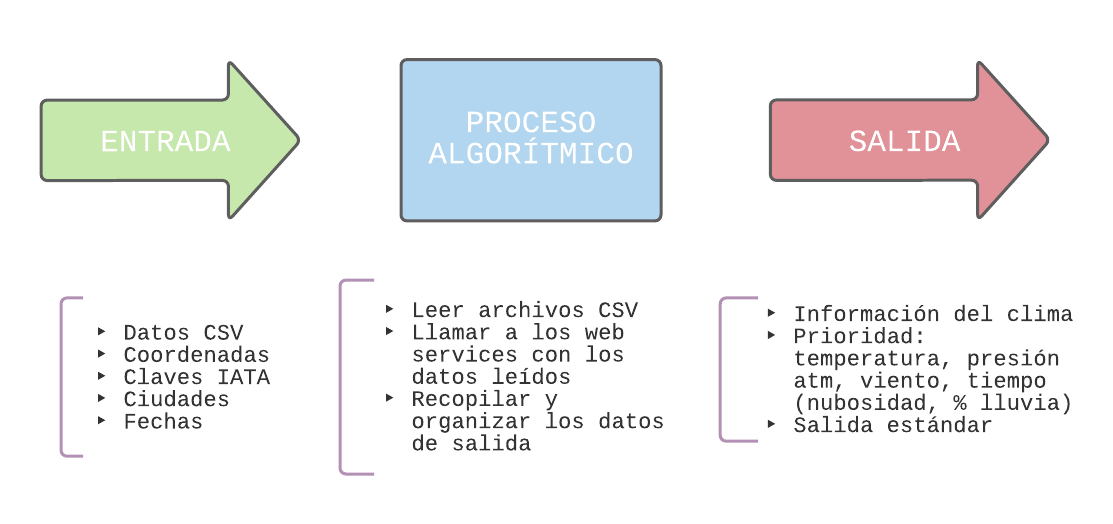
\includegraphics[scale=0.7]{fig1}
			\caption{\small Proceso algorítmico}
		\end{figure}
		
		
		
\section{Diseño del Programa}
		
	Para la implementación del programa, se eligió la orientación a objetos, escribiendo en Ruby, como mencionamos anteriormente. A rasgos generales, queremos que el programa haga lo siguiente:
		
	\begin{enumerate}
		\item Hacer parsing de los archivos CSV dados, sacando los datos en un objeto tipo tabla.
		
		\item Tomar los datos de la tabla uno por uno, y revisar la entrada.
		
		\begin{enumerate}
			\item Si el dato de entrada (código IATA) no se puede leer (está mal escrito), se pasa al siguiente dato de la misma entrada (coordenadas).
			
						\item Si el dato de las coordenadas no funciona tampoco, se imprime un mensaje de error y se pasa al siguiente dato.
				
		\end{enumerate}
			
		\item Si el dato de entrada es válido, se compara con los demás datos del caché.
			
		\begin{enumerate}
			\item Si el dato de entrada coincide con algún dato del caché, se devuelve la información ya almacenada.
				
		\end{enumerate}
				
		\item En caso contrario, se hace la petición al web service para que devuelva la información de clima correspondiente. 
			
		\item Dada la información, se almacena junto con el dato de entrada en el caché para futura referencia.
			
		\item Se imprimen la información a salida estándar.
			
		\item Se repite al algoritmo hasta acabar de leer los archivos.
			
	\end{enumerate}
		
	Se puede visualizar el comportamiento esperado del programa en el siguiente diagrama de flujo.
		
	\begin{figure}[h]
		\centering
   	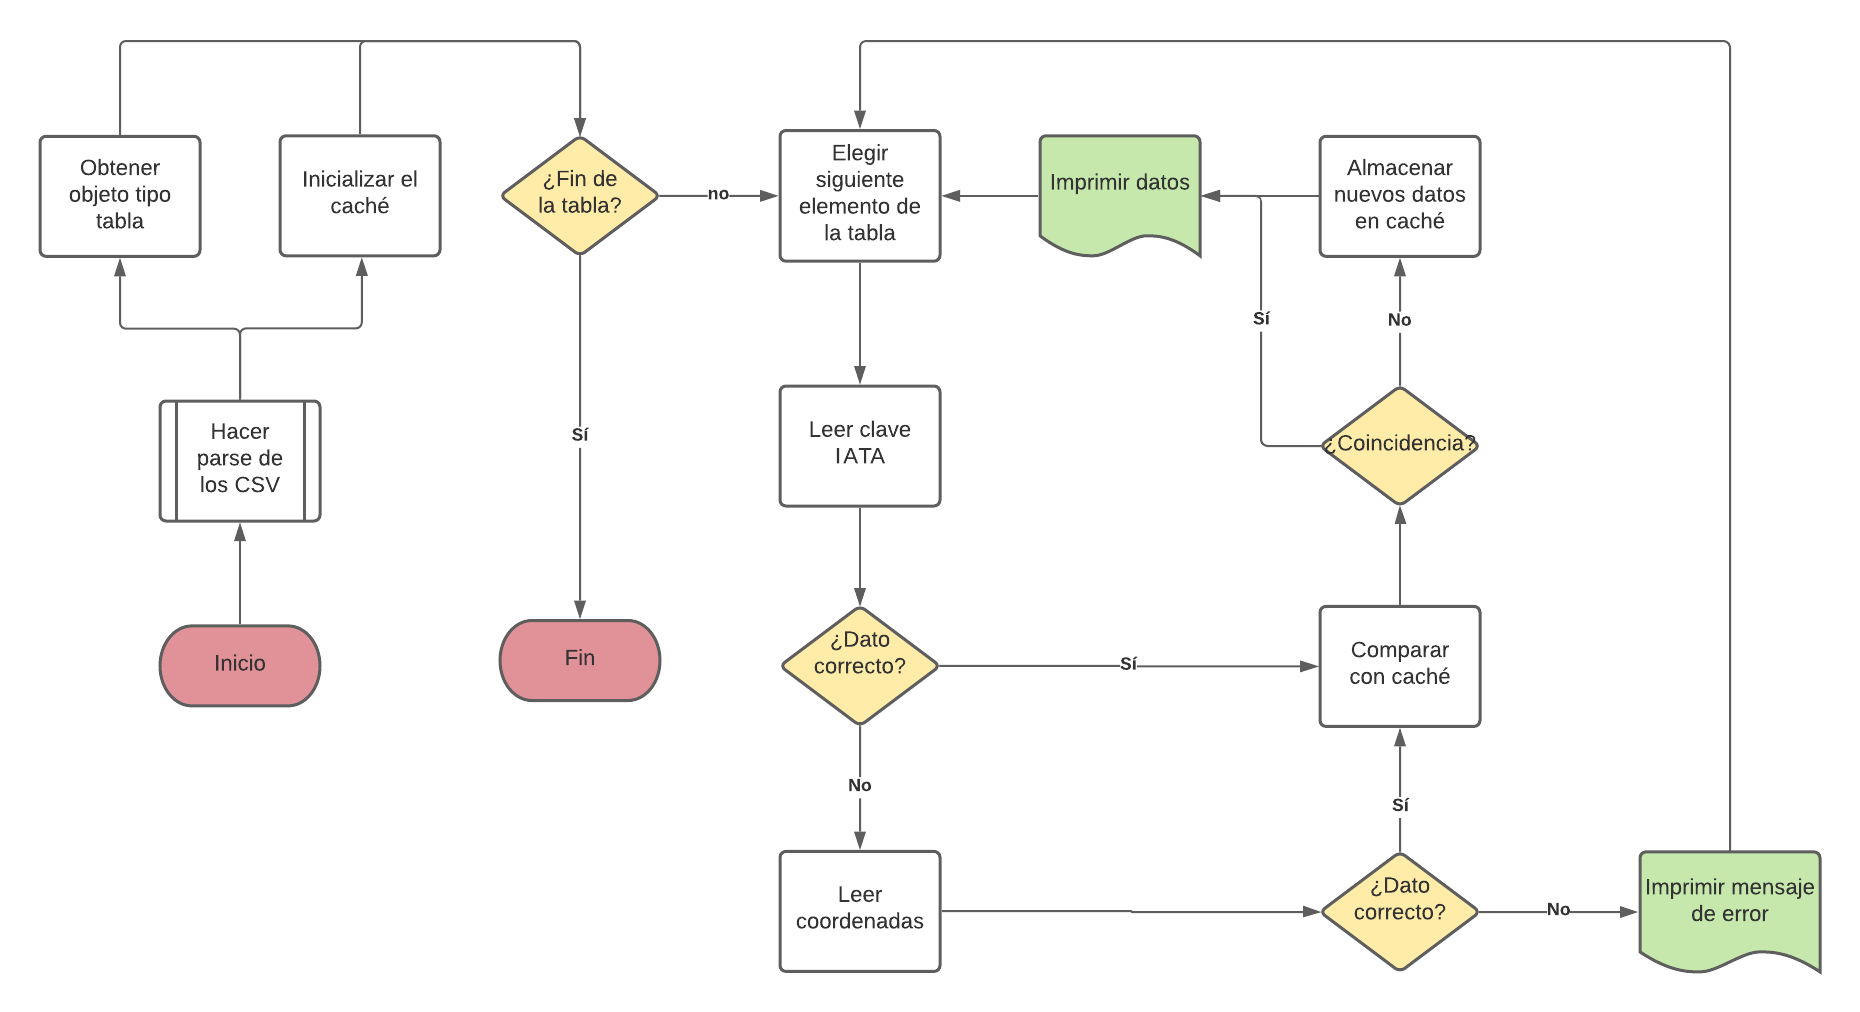
\includegraphics[scale=0.5]{fig2}
		\caption{\small Diagrama de flujo del diseño propuesto}
	\end{figure}
	
	\subsection{TDAs}
	
		Para implementar el proyecto, se eligió el siguiente diseño de clases:
		
		\begin{enumerate}
			\item Una clase que se encargue de hacer el parsing/lectura de los archivos 
		
			\item Una clase que se encargue de hacer las peticiones al web , así como modelar el caché
	
			\item Una clase \emph{main} que inicializa las clases y corre el programa.
		\end{enumerate}
	
		Los TDAs quedarían como sigue:
	
		\begin{figure}[h]
			\centering
   		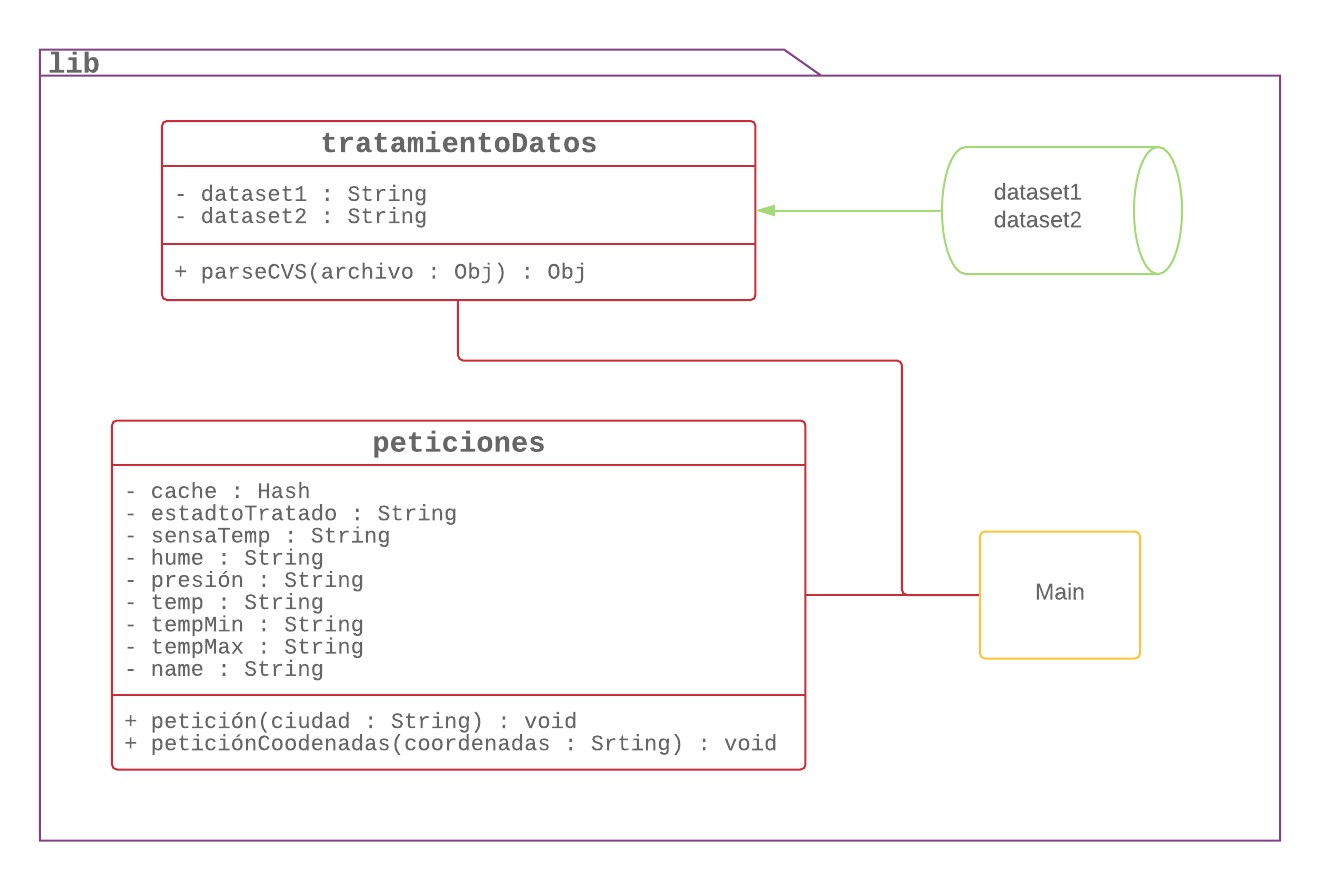
\includegraphics[scale=0.6]{fig3}
			\caption{\small Diagrama de clases del diseño propuesto}
		\end{figure}
	
		Para correr el programa, se utiliza una clase \emph{main}. A continuación mostramos el pseudocódigo de esta clase:

		\begin{lstlisting}[caption={Pseudocódigo de la clase \emph{main}}]
class Main
	petición = petición.new
	td = tratamientoDatos.new

	#Peticiones del dataset1
  for i in 1 .. td.dataset1.length #Longitud de la tabla 1
  	# Variables de cada entrada
    origen = td.parsecsv(dataset1)[i][0]
    destino = td.parsecsv(dataset1)[i][1]
    deslat = td.parsecsv(dataset1)[i][4]
    deslon = td.parsecsv(dataset1)[i][5]

    # Imprimir los datos
    print "Origen: " + origen
    print "Destino: " + destino
    print peticion.peticionCiudad(destino, deslat, deslon)
  end

  #Peticiones del dataset2
  for i in 1 .. td.dataset2.length #Longitud de la tabla 2
  	# Variable de cada entrada
  	destinoInternacional = td.parsecsv(dataset2)[i][0]

  	# Imprimir los datos
    puts "Destino: " + destinoInternacional
    puts peticion.peticionPais(destinoInternacional)
  end
end\end{lstlisting}

		~
		
		La implementación final de las clases se puede revisar en el proyecto.
		
		
\section{Mantenimiento y Costo}

	Considerando los requisitos funcionales, el diseño del programa y el tiempo de implementación, aproximamos una cotización en un rango sugerido de \$8,000.00 - \$12,000.00 pesos mexicanos. Esto incluye código fuente documentación y pruebas unitarias, además, claro, que se garantiza que se cumple con los requisitos.
	
	Sin embargo, viendo a futuro y considerando futuras actualizaciones o mantenimiento, podemos sugerir las siguientes opciones:
	
	\begin{enumerate}
		\item En caso de necesitarse otros formatos de los archivos de entrada, ya sea CSV o algún otro tipo, sería necesario hacer las modificaciones para poder tratar con los datos en el nuevo formato.
		
		\item Implementar una interfaz gráfica para hacer el programa interactivo y más amigable al usuario.
		
		\item Considerar otros tipos de tickets, como vuelos con escalas, conexiones, etc.

	\end{enumerate}

	Tomando en cuenta estas actualizaciones, consideramos un rango de precio parecido al inicial, en dado caso de que se necesite implementarlas en conjunto. Evidentemente, esta apreciación sigue sujeta a un análisis más extenso de estos nuevos requerimientos, y puede cambiar.
	
	
\end{document}
